\documentclass [xcolor=svgnames, t] {beamer} 
\usepackage[utf8]{inputenc}
\usepackage{booktabs, comment} 
\usepackage[absolute, overlay]{textpos} 
\usepackage{pgfpages}
\usepackage[font=footnotesize]{caption}
\useoutertheme{infolines} 



%\definecolor{brownbrown}{RGB}{56, 28, 0}
%\definecolor{brownred}{RGB}{228, 0, 43}

%\setbeamercolor{title in head/foot}{bg=brownred, fg=brownbrown}
%\setbeamercolor{author in head/foot}{bg=myuniversity}
\setbeamertemplate{page number in head/foot}{}
\usepackage{csquotes}


\usepackage{amsmath}
\usepackage[makeroom]{cancel}


\usepackage{textpos}

\usepackage{tikz}

%\tikzset{
%  every overlay node/.style={
%    draw=black,fill=white,rounded corners,anchor=south west,
%  },
%}
% Usage:
% \tikzoverlay at (-1cm,-5cm) {content};
% or
% \tikzoverlay[text width=5cm] at (-1cm,-5cm) {content};
%\def\tikzoverlay{%
%   \tikz[baseline,overlay]\node[every overlay node]
%}%
\tikzset{
  every overlay node/.style={
    anchor=north west,
  },
}
\def\tikzoverlay{%
   \tikz[baseline,overlay]\node[every overlay node]
}%


\newenvironment{smallgreentext}{\scriptsize\color{green}}{\par}
\newenvironment{smallbluetext}{\scriptsize\color{blue}}{\par}
\def\checkmark{\tikz\fill[scale=0.4](0,.35) -- (.25,0) -- (1,.7) -- (.25,.15) -- cycle;}
\usetheme{Madrid}
%\definecolor{myuniversity}{RGB}{56, 28, 0}
%\usecolortheme[named=myuniversity]{structure}

\title[Estructura del documento]{Clase No.03: Estructura del documento}
\subtitle{Revisi\'on de la plantilla del documento}
\institute[]{Departamento de Ingenier\'ia Civil y Agr\'icola\\ Facultad de Ingenier\'ia  \\Universidad Nacional de Colombia - Sede Bogot\'a}
\titlegraphic{
\includegraphics[height=2.0cm]{escudoUnal.png}}
\author[LAM]{Luis Alejandro Morales \\ \href{https://lamhydro.github.io}{https://lamhydro.github.io}}
%\date{\today}
\date{}


\addtobeamertemplate{navigation symbols}{}{%
    \usebeamerfont{footline}%
    \usebeamercolor[fg]{footline}%
    \hspace{1em}%
    \insertframenumber/\inserttotalframenumber
}

\begin{document}
\begin{frame}
\maketitle
\end{frame}


%%%%%%%%%%%%%%%%%%%%%%%%%%%%
\logo{\vspace{-0.2cm}
\includegraphics[height=0.8cm]{escudoUnal.png}~%
}
%%%%%%%%%%%%%%%%%%%%%%%%%%



\begin{frame}
\frametitle{Table of Contents}
\tableofcontents
\end{frame}


%%%%%%%%
\section{Normatividad}
\begin{frame}{Normatividad}
\vspace{-0.3cm}
\centering

\includegraphics[width=\textwidth]{norm}
\small{Articulo 20: \emph{Contenido del Documento de Proyecto de T\'esis de Maestr\'ia}}
\centering

\includegraphics[width=\textwidth]{norm1}
\end{frame}
\begin{frame}{Normatividad}
\centering
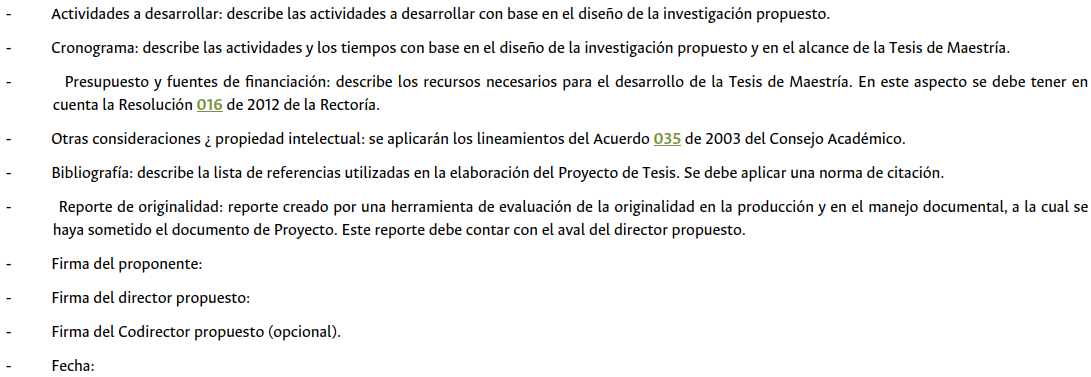
\includegraphics[width=\textwidth]{norm2}
\end{frame}

%%%%%%%%
\section{Indice general de un documento de tesis or proyecto}

\begin{frame}{Indice del documento}
\begin{columns}[T]
\column{0.3\textwidth}
El indice de un trabajo final de maestria, es la \alert{carta de navegacion del proyecto}. Esta puede cambiar y se puede modificar de acuerdo con las necesidades que surjan en la realizacion del proyecto. 
\column{0.7\textwidth}
\centering
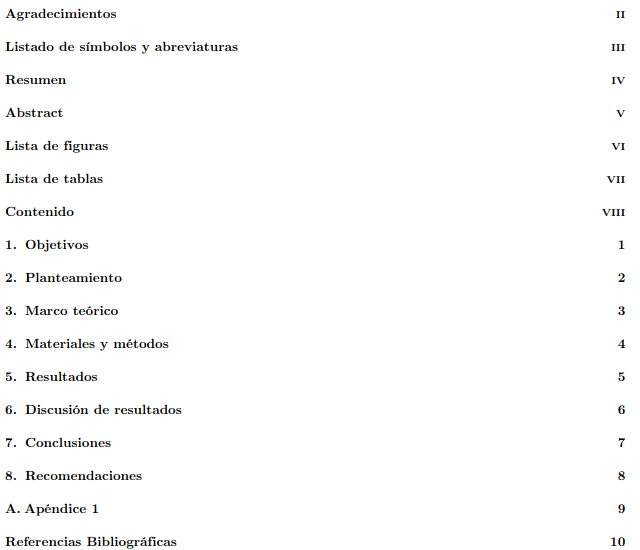
\includegraphics[width=\textwidth]{thesisIndx}
\end{columns}
\tikzoverlay[text width=3cm] at (5.1cm,5.2cm) {
\begin{smallgreentext}
(\href{https://bibliotecas.unal.edu.co/servicios/servicios-en-linea/entrega-de-tesis-y-publicaciones-en-linea}{https://bibliotecas.unal.edu.co/servicios/servicios-en-linea/entrega-de-tesis-y-publicaciones-en-linea})
\end{smallgreentext}
};
\end{frame}


\begin{frame}{Indice del documento}
Estructura general de un documento de proyecto de tesis:
\begin{columns}[T]
\column{0.2\textwidth}
\scriptsize{
\begin{itemize}
\item T\'itulo
\item Resumen
\item Introducci\'on
\item Metodolog\'ia 
\item Resultados
\item Discusion
\item Conclusiones
\item Bibliograf\'ia
\item Anexos
\end{itemize}
}
\column{0.4\textwidth}
\centering
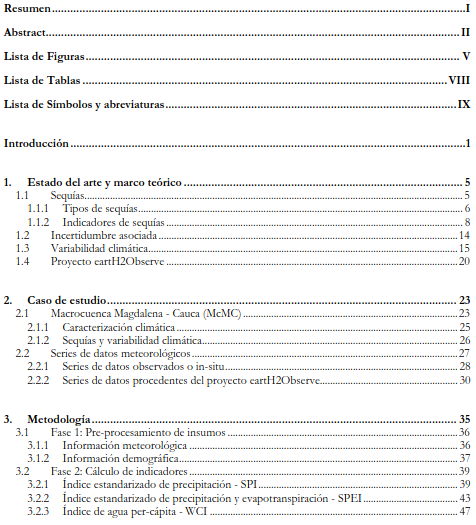
\includegraphics[width=\textwidth]{idx1}
\column{0.4\textwidth}
\centering
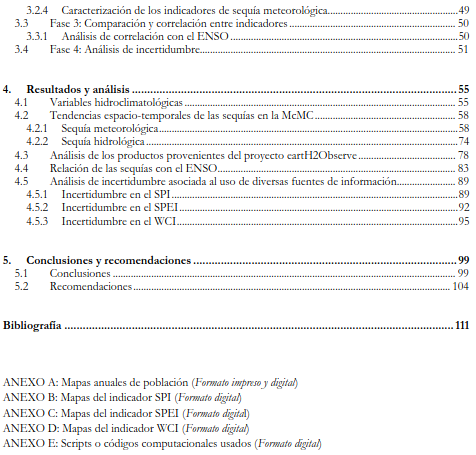
\includegraphics[width=\textwidth]{idx2}
\end{columns}
\tikzoverlay[text width=3cm] at (3cm,0cm) {
\begin{smallgreentext}
(\href{https://repositorio.unal.edu.co/handle/unal/69784}{https://repositorio.unal.edu.co/handle/unal/69784})
\end{smallgreentext}
};
\end{frame}
%%%%%%%%

\section{Estructura del documento}
\begin{frame}{Titulo}
El titulo debe reflejar y ser congruente con el \alert{objetivo principal}. El t\'itulo debe cumplir dos funciones:
\begin{itemize}
\item \alert{Atraer} a otros para leer el documento
\item Proporcionar la \alert{mejor informacion posible} para, e.j. agilizar la busqueda
\end{itemize}
\emph{¿Como construir un buen titulo?}
\begin{enumerate}
\item Escoger las \alert{palabras claves} en su proyecto.
\item Ordernar las palabras claves de acuerdo con su \alert{importancia}.
\item Construya el titulo colocando las \alert{palabras} de acuerdo con el \alert{orden de importancia}.
\item Si el titulo es \alert{muy largo}, \alert{borre} las palabras menos importantes. 
\end{enumerate}
\tikzoverlay[text width=12cm] at (1cm,0.5cm) {
\begin{smallgreentext}
The influence of season of calving on the performance of Holstein cows.
\end{smallgreentext}
\begin{smallbluetext}
Holstein cows produce more milk if they calve in spring instead of autumn. \checkmark
\end{smallbluetext} 
};
\end{frame}

\begin{frame}{Resumen}
\tikzoverlay[text width=12.5cm] at (-0.2cm,0.8cm) {
\begin{smallbluetext}
"Please be goog enough to put your conclusions and recomendations on one sheet of paper at the very beginning of your report, so that I can even consider reading it" Winston Churchill
\end{smallbluetext} 
};
\begin{minipage}[t]{1.03\textwidth} 
Es una \alert{mini t\'esis} o trabajo. Generalmente es lo que primero y lo que \alert{m\'as se lee} despu\'es del t\'itulo. Caracter\'isticas del resumen:
\begin{itemize}
\item Debe escribirse en \alert{Espa\~nol} y en \alert{Ingl\'es}.
\item Debe incluir las \alert{palabras claves}.
\item Debe incluir entre \alert{150 y 250 palabras}.
\end{itemize}
Componentes esenciales de un resumen
\begin{enumerate}
\item ¿Cual es la motivaci\'on o justificaci\'on del proyecto? \alert{¿Porqu\'e?}
\item ¿Que metodologia, sitio de estudio y datos se usaron en el proyecto? \alert{¿C\'omo?}
\item ¿Que se encontro (resultados) despues de desarrolar el proyecto? \alert{Resultados principales}
\item ¿Cual es la conclusi\'on con base en los resultados encontrados?\alert{Conclusion principal}
\end{enumerate}
\end{minipage}
\end{frame}

\begin{frame}{Bad and good abstracs}
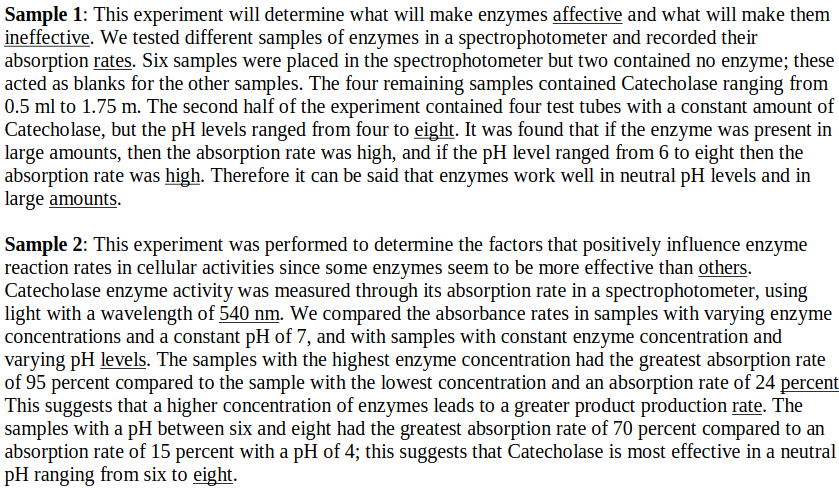
\includegraphics[width=0.9\textwidth]{badGood}
\tikzoverlay[text width=1.5cm] at (-0.2cm,6cm) {

\includegraphics[width=\textwidth]{X}
};
\tikzoverlay[text width=1.5cm] at (-0.3cm,2.8cm) {

\includegraphics[width=\textwidth]{chm}
};
\end{frame}

\begin{frame}{Introducci\'on}

\end{frame}


%\begin{frame}{Indice de un documento}
%\tikzoverlay[text width=4cm] at (0cm,3cm) {
%  \begin{itemize}
%  \item \emph{Derive subclass} from \texttt{GetOptWrapper}
%  \item one \emph{variable definition} per option
%  \item \emph{Default Values}ccccccccc cccccccc cccccccc ccccccc cccccccc ccccccc
%  \end{itemize}
%};
%%\begin{tikzpicture}
%%  \node (A) at (0,0) {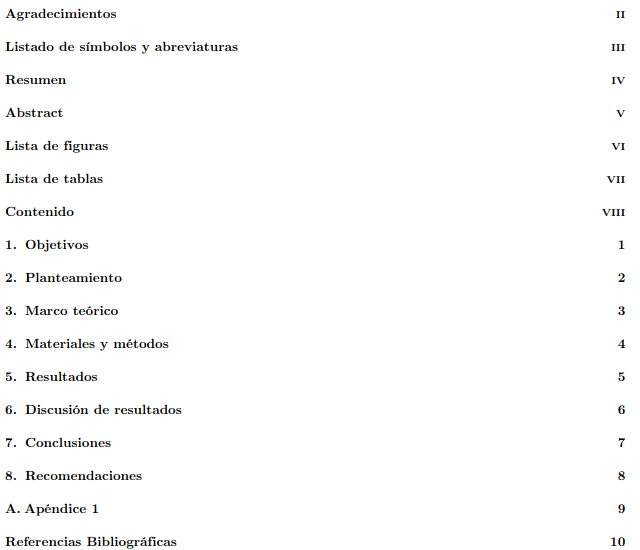
\includegraphics[width=3cm]{thesisIndx}};
%%  \node [below of=A] {My caption};
%%  \node (B) at (3,0.5) {
\includegraphics{escudoUnal}};
%%  \node [below of=B] {My second caption};
%%  \node (C) at (1,1) {sdfaaaaaaaaaaaaaaaaaaaaaaaaaaaaaaaaaaaaaaaaaaaaaaaaaaaaaaaaaaaaaaaaaaaaaaaaaaaaaaaaaaaaaaaaaaaaaaaaaaaaaaaaaaaaaaaaaaaaaaaaaaaaaaaa};
%%\end{tikzpicture}
%\begin{tikzpicture}[remember picture]
%    \node[xshift=-0.6cm,yshift=-0.8cm] at (current page.north east) {
\includegraphics{escudoUnal.png}};
%\end{tikzpicture}
%\tikzoverlay[text width=2cm] at (-3cm,-3cm) {saddddddddddddddddddddddddddddddddddddddddddddddddddddd};
%\end{frame}

%%%%%%%%


%%%%%%%% %\begin{frame} [allowframebreaks]\frametitle{References}
%        \bibliographystyle{apalike}
%        \bibliography{bibfile}
%\end{frame}

\end{document}

